\chapter{Cơ sở lý thuyết}
\label{chapter2}
Chương \ref{chapter2} em sẽ trình bày những kiến thức và các công cụ cần có để xây dựng một website mà em tìm hiểu được để phục vụ cho những vấn đề nêu ra ở chương \ref{chapter1}
\section{Ngôn ngữ lập trình C\# } \label{ngonngu} 
C\# là một ngôn ngữ lập trình hướng đối tượng được phát triển bởi Microsoft, là phần khởi đầu cho kế hoạch .NET của Microsoft. Tên của ngôn ngữ bao gồm ký tự thăng theo Microsoft nhưng theo ECMA là C\#, chỉ bao gồm dấu số thường. Microsoft phát triển C\# dựa trên C++ và Java. C\# được miêu tả là ngôn ngữ có được sự cân bằng giữa C++, Visual Basic, Delphi và Java.
\par
C\# được thiết kế chủ yếu bởi Anders Hejlsberg kiến trúc sư phần mềm nổi tiếng với các sản phẩm Turbo Pascal, Delphi, J++, WFC.
Tiêu chuẩn ECMA liệt kê các mục tiêu của việc thiết kế ngôn ngữ C\#:
\begin{itemize}
\item Ngôn ngữ được dự định là một ngôn ngữ lập trình đơn giản, hiện đại, hướng đến nhiều mục đích sử dụng, và là một ngôn ngữ lập trình hướng đối tượng.
\item Ngôn ngữ và việc triển khai đáp ứng các nguyên tắc của ngành kỹ thuật phần mềm như kiểm tra chặt chẽ kiểu dữ liệu, kiểm tra giới hạn mảng, phát hiện các trường hợp sử dụng các biến chưa có dữ liệu, và tự động thu gom rác. Tính mạnh mẽ, sự bền bỉ, và năng suất của việc lập trình là rất quan trọng đối với ngôn ngữ này.
\item Ngôn ngữ sẽ được sử dụng để phát triển các thành phần của phần mềm theo hướng thích hợp cho việc triển khai trong các môi trường phân tán.
\item Khả năng di chuyển (portability) là rất quan trọng, đặc biệt là đối với những lập trình viên đã quen với C và C++.
\item Hỗ trợ quốc tế hóa.
\item Ngôn ngữ sẽ được thiết kế để phù hợp với việc viết các ứng dụng cho cả hai hệ thống: hosted và nhúng, từ các phần mềm quy mô lớn, đến các phần mềm chỉ có các chức năng đơn giản.
\item Mặc dù các ứng dụng C\# có tính kinh tế đối với các yêu cầu về bộ nhớ và chế độ xử lý, ngôn ngữ này không cạnh tranh trực tiếp về hiệu năng và kích thước đối với ngôn ngữ C hoặc assembly
\item C\# được biên dịch ra mã trung gian MSIL sau đó thực thi bởi Common Language Runtime (CLR) \cite{2}.
\end{itemize}
\par
Em chọn ngôn ngữ C\# bởi vì:
\begin{itemize}
\item Rất phổ biến và được sử dụng bởi hàng triệu lập trình viên trên toàn thế giới.
\item Dễ học và sử dụng.
\item So với Java thì nó là đối thủ lớn nhất. Chúng ta không so sánh 2 ngôn ngữ nhưng em thích C\# vì nó luôn cải tiến.
\item Nền tảng .NET cũng luôn phát triển ngày càng hiện đại trong khi Java phát triển chậm.
\end{itemize}

\section{.NET}
.NET bao gồm 3 thành phần:
\begin{itemize}
\item Runtime
\item Libraries
\item Toolings
\end{itemize}
\par
Quy trình biên dịch và chạy chương trình của .NET. Hình \ref{refhinh2_2} ta thấy từ source code qua trình biên dịch tương ứng của ngôn ngữ đấy trong hệ sinh thái .NET ví dụ như C\# compiler hay VB.NET compiler để sinh ra MSIL code.  Ngôn ngữ trung gian trong .NET nó khá gần với mã máy nhưng không chứa thông tin cụ thể về CPU, nên ngôn ngữ MSIL giúp cho đoạn code trung gian của chúng ta có thể hoạt động trên nhiều loại CPU (64bit, 32bit), cũng như nhiều loại kiến trúc khác nhau (ARM, Intel…). Trên thực tế một vài ngôn ngữ (Javascript, Python…) không sử dụng đến ngôn ngữ trung gian: Source sẽ được dịch thẳng ra mã máy tại ‘Runtime’. Điểm lợi của việc này là quá trình build được đơn giản hóa, tuy nhiên hiệu năng sẽ bị hạn chế.
Ngoài việc biên dịch, môi trường hoạt động (Runtime) còn có những công dụng như:
\begin{itemize}
\item Tự động quản lý bộ nhớ. Khi làm việc với những ngôn ngữ bậc cao như C\# hay Java, chúng ta không cần  giải phóng bộ nhớ bằng cách gọi free() như khi làm việc với C/C++. CLR bao gồm một công cụ dọn rác (Garbage collector -GC) sẽ tự động giải phóng những phần bộ nhớ không được sử dụng
\item Strong typings: CLR quản lý thông tin về các kiểu dữ liệu đã sử dụng. Điều này giúp cho lập trình viên có thể phân biệt được các định dạng thông tin của từng biến khác nhau (class, structure…)
\end{itemize}
\par
Khi làm việc với .NET, code của chúng ta sẽ tương tác với rất nhiều các class khác nhau. Tất cả những class này được định nghĩa trong hệ thống thư viện cơ bản của .NET được gọi tắt là BCL (Base class libraries). Mã nguồn của BCL, trái với mọi người hay nghĩ, là mã nguồn mở. Chúng ta có thể truy cập mã nguồn này tại sourceof.net. Các công cụ (toolings) của .NET bao gồm compiler và Visual Studio .NET sử dụng hệ thống build của Microsoft gọi là MSBuild. Đối với nền tảng .NET core mới thì chúng ta còn có thêm công cụ dòng lệnh (dotnet cli).
\begin{center}
    \begin{figure}[h]
    \begin{center}
     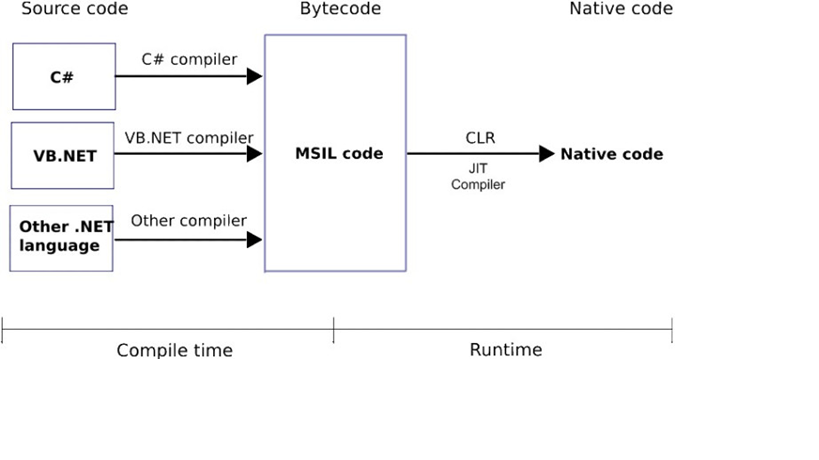
\includegraphics[scale=0.6]{image/chayDotNet.png}
    \end{center}
    \caption{Quy trình biên dịch và chạy chương trình}
    \label{refhinh2_2}
    \end{figure}
\end{center}
\par
Hình \ref{refhinh2_3} chúng ta có thể thấy về cơ bản, .NET Framework, .NET core và Mono là ba phiên bản .NET khác nhau (có nghĩa là mỗi phiên bản có Runtime, Libraries và Toolings riêng).
\begin{center}
    \begin{figure}[h]
    \begin{center}
     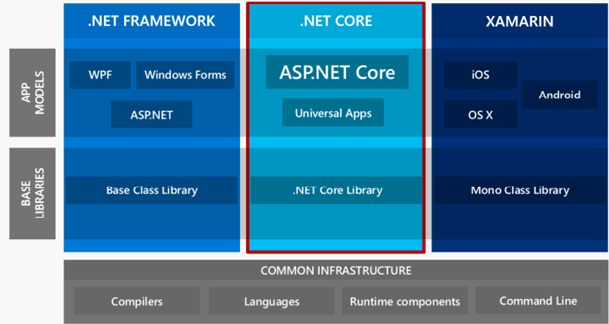
\includegraphics[scale=0.9]{image/kienTrucDotNetCore.png}
    \end{center}
    \caption{Kiến trúc của .NET }
    \label{refhinh2_3}
    \end{figure}
\end{center}
\begin{itemize}
\item .NET Framework được Microsoft đưa ra chính thức từ năm 2002. .NET Framework chỉ hoạt động trên Windows. Những nền tảng ứng dụng như WPF, Winforms, ASP.NET(1-4) hoạt động dựa trên .NET Framework.
\item Mono là phiên bản cộng đồng nhằm mang .NET đến những nền tảng ngoài Windows. Mono được phát triển chủ yếu nhằm xây dựng những ứng dụng với giao diện người dùng và được sử dụng rất rộng rãi: Unity Game, Xamarin…
\item Cho đến năm 2013, Microsoft định hướng đi đa nền tảng và phát triển .NET core. .NET core hiện được sử dụng trong các ứng dụng Universal Windows platform và ASP.NET Core.
\item Tuyệt đối không nên dùng Mono để vận hành webserver. Bộ máy dọn rác của Mono không được thiết kế để hoạt động với webserver và sẽ gây ra quá tải nhanh chóng
\item Nên lựa chọn .NET Framework hay .NET Core cho các web server .NET Core chạy được đa nền tảng và có hiệu năng cao hơn. Nhược điểm duy nhất của nó là số lượng thư viện hỗ trợ vẫn còn hạn chế. .NET Framework có hệ sinh thái lớn hơn với nhiều các thư viện hỗ trợ hơn.
\end{itemize}

\subsection{.NET Framework}
Như đã nêu ở phần \ref{ngonngu} ngôn ngữ C\# ra đời để phục vụ Microsoft phát triển nền tảng .NET Framework phục vụ phát triển cho nhiều ứng dụng cho nên C\# không đứng riêng lẻ mà nó là 1 phần của nền tảng .NET, .NET Framework bao gồm môi trường phát triển, hỗ trợ đa ngôn ngữ mà C\# là một trong số đó (ngoài ra có F\#, VB.NET, Managed C++, J\#).
Những thành phần của .NET Framework (Hình \ref{refhinh2_1}) bao gồm:
\begin{itemize}
\item Các ngôn ngữ lập trình .NET (C\#, VB.NET…).
\item Môi trường thực thi code (CLR) sẽ thực thi chương trình được viết từ ngôn ngữ lập trình.
\item Các công cụ phát triển như trình biên dịch CSC dùng để biên dịch ngôn ngữ C\# sang mã trung gian (MSIL) mà CLR có thể hiểu.
\item Tập các thư viện chuẩn (Class Library) như ADO.NET cho phép truy cập database (ví dụ SQL Server hoặc MySQL) và WCF cho phép tạo ra các ứng dụng API theo chuẩn HTTP và trả về JSON, SOAP…
\end{itemize}
\par
.Net Framework hiện tại là phiên bản hỗ trợ nhiều ứng dụng nhất khi nó có thể dùng để viết các ứng dụng chạy trên nền Windows như: Web App, Win App hay là nó có thể xây dựng những tầng Web API giành cho nền tảng Web hay Mobile.
\begin{center}
    \begin{figure}[h]
    \begin{center}
     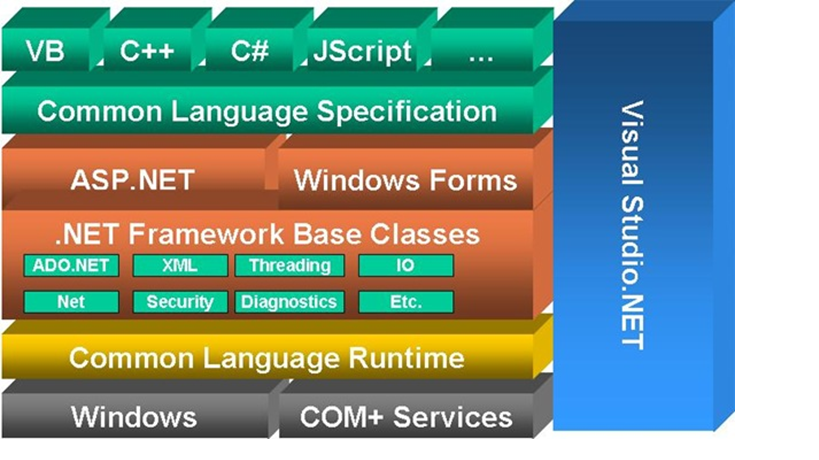
\includegraphics[scale=0.6]{image/kienTrucDotNet.png}
    \end{center}
    \caption{Kiến trúc .Net Framework}
    \label{refhinh2_1}
    \end{figure}
\end{center}
\subsection{Mono}
Mono là một nền tảng open-source với mục đích chính là tạo những ứng dụng cross-platform trên nền .Net. Chúng ta có thể sử dụng Mono trên các hệ điều hành như Unix, Linux, Mac OS X, Solaris và tất nhiên là Windows. Bất kì ngôn ngữ nào được biên dịch thành mã IL thuần túy đều có thể tương thích với Mono. Ngoài ra, Mono còn cung cấp thư viện hỗ trợ rất nhiều loại ngôn ngữ lập trình khác như Java, PHP, Python, Object Pascal, Cobra… Mono framework được sử dụng để lập trình ứng dụng mobile và game 2D, 3D. Các thành phần chính của Mono Framework:
\begin{itemize}
\item Mono runtime: cung cấp trình biên dịch Just-in-Time (JIT), Ahead-of-Time (AOT), thực thi, quản lý các tiến trình và giao tiếp với hệ thống.
\item C\# Compiler: bao gồm các công cụ
\begin{itemize}
\item mcs: (phiên bản 1.1) hỗ trợ C\# 1.0 và C\# 3.0 ngoại trừ các tính năng về generic.
\item gmcs: (phiên bản 2.0) hỗ trợ đầy đủ C\# 3.0.
\item smcs: (phiên bản 2.1) hỗ trợ thêm Silverlight/Moonlight.
\item dmcs: (phiên bản 4.0) hỗ trợ C\# 4.0.
\end{itemize}
\item Base Class Library: thư viện nền tảng để phát triển ứng dụng, tương thích với .Net framework.
\item Mono Class Library: Cung cấp các thư viện lập trình như Gtk+, Zip files, LDAP, OpenGL, Cairo, POSIX,… \cite{4}
\end{itemize}
\subsection{.NET Core}
.NET Core là một framework mã nguồn mở mới và framework đa nền tảng (cross-platform) cho việc xây dựng những ứng dụng hiện tại dựa trên kết nối đám mây, giống như web apps, IoT và backend cho mobile. Ứng dụng ASP.NET Core có thể chạy trên .NET Core hoặc trên phiên bản đầy đủ của .NET Framework. Nó được thiết kế để cung cấp và tối ưu hệ thống đang và đã phát triển cho những ứng dụng được triển khai trên đám mây (cloud) hoặc chạy on-promise. Nó bao gồm các thành phần theo hướng module nhằm tối thiểu tài nguyên và chi phí phát triển. Chúng ta có thể phát triển và chạy những ứng dụng ASP.NET Core đa nền tảng trên Windows, Mac và Linux. Đồng thời nó đã trở thành một mã nguồn mở. Đây là một thay đổi rất lớn và theo em là quan trọng nhất của ASP.NET Core. Điều mà trước đây khó có một lập trình viên nào có thể nghĩ đến. Có lẽ đó cũng là một xu thế mà các ngôn ngữ lập trình hiện nay đang hướng tới.
\par
Bản phát hành đầu tiên của ASP.NET đã xuất hiện cách đây 15 năm trước, nó là một phần của .NET Framework. Từ đó, hàng triệu lập trình viên đã sử dụng nó để xây dựng những ứng dụng web tuyệt vời, và trên những năm đó Microsoft đã phát triển thêm nhiều tính năng mới.ASP.NET Core có một số thay đổi kiến trúc lớn, đó là kết quả của việc học hỏi rất nhiều từ các framework module hóa khác. ASP.NET Core không còn dựa trên System.Web.dll nữa. Nó được dựa trên một tập hợp các gói, các module hay cũng được gọi là các Nuget packages. Điều này cho phép chúng ta tối ưu ứng dụng để chỉ bao gồm những packages nào cần thiết. Lợi ích của nó là giúp cho ứng dụng nhỏ hơn, bảo mật chặt chẽ hơn, giảm sự phức tạp, tối ưu hiệu suất hoạt động và giảm chi phí, thời gian cho việc phát triển. Với ASP.NET Core chúng ta đạt được những nền tảng cải tiến dưới đây:
\begin{itemize}
\item Hợp nhất việc xây dựng web UI và web APIs.
\item Tích hợp những client-side frameworks hiện đại và những luồng phát triển.
\item Hệ thống cấu hình dựa trên môi trường đám mây thật sự.
\item Dependency injection được xây dựng sẵn.
\item HTTP request được tối ưu nhẹ hơn.
\item Có thể host trên IIS hoặc self-host trong process của riêng project hiện tại.
\item Được xây dựng trên .NET Core, hỗ trợ thực sự app versioning.
\item Chuyển các thực thể, thành phần, module như những NuGet packages
\item Những công cụ mới để đơn giản hóa quá trình phát triển web hiện đại
\item Xây dựng và chạy đa nền tảng(Windows, Mac và Linux)
\item Mã nguồn mở và tập trung vào cộng đồng
\end{itemize}
\subsection{Vòng đời yêu cầu trong ASP.NET}
Trong ASP.NET có 2 loại vòng đời:
\begin{itemize}
	\item Vòng đời của ứng dụng là quá trình ứng dụng thực sự bắt đầu chạy IIS cho đến khi nó dừng lại. Vòng đời ứng dụng có thể chia thành các giai đoạn sau:
	\begin{itemize}
		\item Người dùng gửi yêu cầu truy cập vào dữ liệu của ứng dụng và trình duyệt sẽ gửi yêu cầu này đến Web Server
		\item Các sự kiện sau đây sẽ được khởi tạo:
		\begin{itemize}
			\item Một đối tượng của lớp ApplicationManager được tạo.
			\item Một đối tượng lớp HostingEvironment được tạo để cung cấp thông tin về nguồn dữ liệu.
			\item Các thành phần đầu của ứng dụng sẽ được biên dịch.
		\end{itemize}
		\item Các đối tượng HttpContext, HttpRequest và HttpResponse được khởi tạo và cài đặt.
		\item Một thể hiện của đối tượng HttpApplication được tạo và gắn cho yêu cầu.
		\item Các yêu cầu được xử lý bởi lớp HttpApplication, các sự kiện khác nhau được kích hoạt bởi lớp này để xử lý các yêu cầu.
	\end{itemize}
	\item Vòng đời của yêu cầu gửi lên server.
\end{itemize}
\begin{center}
    \begin{figure}[h]
    \begin{center}
     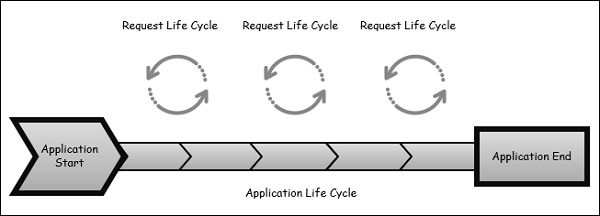
\includegraphics[scale=1.0]{image/vongdoiMVC.png}
    \end{center}
    \caption{Tổng quan vòng đời trong ASP.NET nói chung}
    \label{refhinh2_4}
    \end{figure}
\end{center}
\par
Hình \ref{refhinh2_4} là một vòng đời của một ứng dụng trong nền tảng .NET. Ta có thể thấy trong một vòng đời ứng dụng có rất nhiều các yêu cầu gửi lên từ các user cho server xử lý, mỗi một vòng đời của một yêu cầu gửi lên cho server xử lý sẽ chứa rất nhiều sự kiện mà người dùng thao tác và mong muốn server trả kết quả ra ngoài màn hình. Kết thúc một vòng đời một của yêu cầu hệ thống sẽ tự động đóng kết nối và dọn những thực thể mà yêu cầu đã sử dụng.
\begin{center}
    \begin{figure}[h]
    \begin{center}
     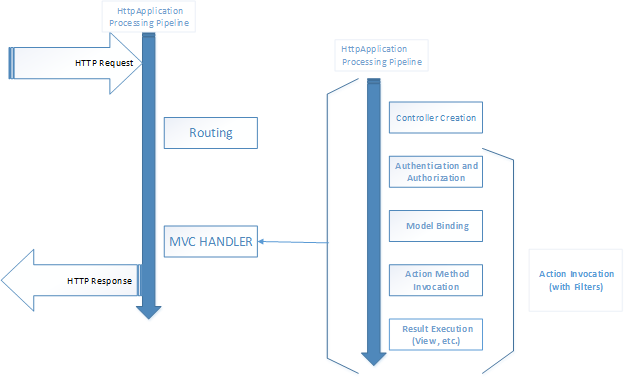
\includegraphics[scale=1.0]{image/vongdoiMVCchitiet.png}
    \end{center}
    \caption{Vòng đời trong ASP.NET MVC}
    \label{refhinh2_5}
    \end{figure}
\end{center}
\par
Hình \ref{refhinh2_5} là hình mô tả chi tiết vòng đời trong ASP.NET MVC ở mức 2 level. Khi có 1 yêu cầu gửi lên ứng dụng sẽ có một chuỗi sự kiện được xử lý ở server, nó sẽ được định tuyến qua 1 đường ống xử lý trong lớp HttpApplication để đến được đúng Controller và Action của nó, khi vào Controller sự kiện đấy phải được kiểm tra quyền đăng nhập và quyền ứng dụng nếu ứng dụng có cài đặt 2 quyền trên, sau đó là bước truyền các tham số vào cho Action xử lý nếu qua được bước kiểm tra quyền cuối cùng Action sẽ trả về 1 kết quả cho Controller gửi ra View và trả về 1 kết quả được hiển thị cho người dùng thông qua View.
\begin{center}
    \begin{figure}[h]
    \begin{center}
     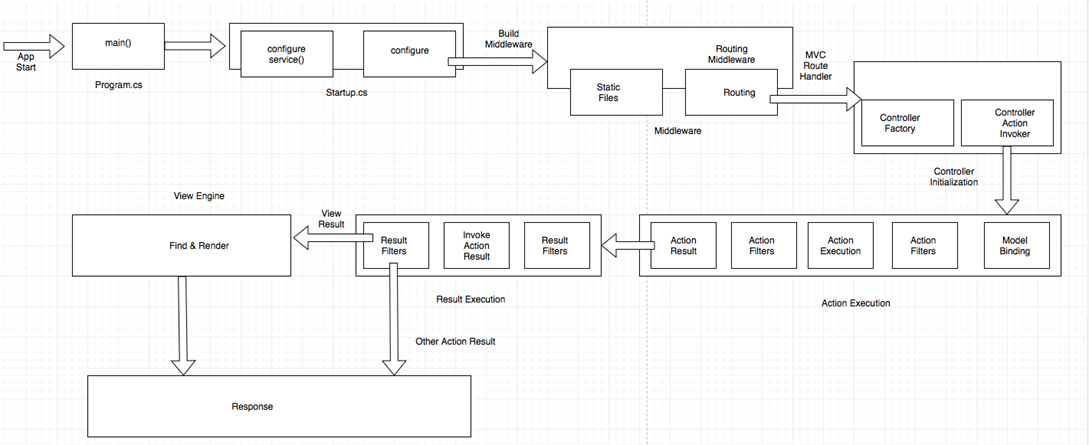
\includegraphics[scale=0.6]{image/vongdoiCore.png}
    \end{center}
    \caption{Vòng đời trong ASP.NET Core}
    \label{refhinh2_6}
    \end{figure}
\end{center}
\par
Hình \ref{refhinh2_6} mô tả chi tiết vòng đời trong ASP.NET Core. Khi có một yêu cầu gửi đến server nó cũng sẽ được định tuyến qua 1 URL nhất định, vì ASP.NET Core được thiết kế theo dạng module hoá nên các module được khởi tạo và sử dụng được khai báo trong file StartUp.cs trong đó phương thức ConfigureServices() để khai báo những module được sử dụng trong hệ thống, còn phương thức Configure() được sử dụng để sử dụng các module đã khai báo. Sau đấy qua tầng Middleware là tầng ở giữa để xử lý định tuyến URL và những file tĩnh trong hệ thống như: file css, js,... Ở tầng Middleware này, lập trình viên có thể lập trình cho hệ thống gửi kèm một số thứ lên cùng với yêu cầu người dùng như là gửi kèm 1 header để xác thực người dùng chẳng hạn. Sau khi định tuyến được yêu cầu thì server xử lý các tham số của yêu cầu vào trong Controller, ở Controller các thể hiện sẽ được tiêm vào hàm tạo của Controller theo cơ chế Dependency Injection. Sau khi xử lý thành công ở Controller thì hệ thống sẽ trả lại kết quả đến hiển thị trên View cho người dùng. 
\section{CSHTML}
CSHTML là 1 view engine dùng để xử lý và tạo HTML, nó là 1 view để nhận các dữ liệu mà controller gửi đến, CSHTML cho phép viết mã nguồn C\# để xử lý dữ liệu trên view dễ dàng hơn. CSHTML sử dụng Raroz để viết mã. Cơ chế Razor giảm thiểu số lượng ký tự và phím nhấn cần để tạo một tập tin View, do đó lập trình viên có thể làm việc nhanh và trôi chảy hơn. Khi chạy trên môi trường web thì file CSHTML sẽ tự động trở thành mã HTML để hiển thị lên các trình duyệt website
\section{Bootstrap}
Bootstrap là 1 framework HTML, CSS, và JavaScript cho phép người dùng dễ dàng thiết kế website theo 1 chuẩn nhất định, tạo các website thân thiện với các thiết bị cầm tay như mobile, ipad, tablet,...
\par
Bootstrap bao gồm những cái cơ bản có sẵn như: typography, forms, buttons, tables, navigation, modals, image carousels và nhiều thứ khác. Trong bootstrap có thêm nhiều Component, Javascript hỗ trợ cho việc thiết kế reponsive của chúng ta dễ dàng, thuận tiện và nhanh chóng hơn. Nên dùng bootstrap để viết giao diện front-end vì:
\begin{itemize}
\item Bootstrap là một trong những framework được sử dụng nhiều nhất trên thế giới để xây dựng nên một website. Bootstrap đã xây dựng nên 1 chuẩn riêng và rất được người dùng ưa chuộng. Chính vì thế, chúng ta hay nghe tới một cụm từ rất thông dụng "Thiết kế theo chuẩn Bootstrap".
\item Rất dễ để sử dụng: Nó đơn giản vì nó được base trên HTML, CSS và Javascript chỉ cần có kiến thức cơ bản về ba ngôn ngữ nêu trên là có thể sử dụng bootstrap tốt.
\item Responsive: Bootstrap xây dựng sẵn reponsive css trên các thiết bị Iphones, tablets, và desktops. Tính năng này khiến cho người dùng tiết kiệm được rất nhiều thời gian trong việc tạo ra một website thân thiện với các thiết bị điện tử, thiết bị cầm tay.
\item Tương thích với trình duyệt: Nó tương thích với tất cả các trình duyệt (Chrome, Firefox, Internet Explorer, Safari, and Opera). Tuy nhiên, với IE browser, Bootstrap chỉ hỗ trợ từ IE9 trở lên. Điều này vô cùng dễ hiểu vì IE8 không support HTML5 và CSS3.
\end{itemize}

\section{Jquery Ajax}
\subsection{Jquery}
jQuery là một Framework được xây dựng dựa trên các tính năng của JavaScript. Vì thế trong khi phát triển các ứng dụng sử dụng jQuery, chúng ta có thể sử dụng tất cả các hàm và các tính năng khác được bổ trợ trong JavaScript. jQuery làm đơn giản hóa việc truyền tải HTML, xử lý sự kiện, tạo hiệu ứng động và tương tác Ajax. Với jQuery, khái niệm Rapid Web Development đã không còn quá xa lạ. jQuery là một bộ công cụ tiện ích JavaScript làm đơn giản hóa các tác vụ đa dạng với việc viết ít code hơn. Dưới đây liệt kê một số tính năng tối quan trọng được hỗ trợ bởi jQuery:
\begin{itemize}
\item Thao tác DOM: jQuery giúp dễ dàng lựa chọn các phần tử DOM để traverse (duyệt) một cách dễ dàng như sử dụng CSS, và chỉnh sửa nội dung của chúng bởi sử dụng phương tiện Selector mã nguồn mở, mà được gọi là Sizzle.
\item Xử lý sự kiện: jQuery giúp tương tác với người dùng tốt hơn bằng việc xử lý các sự kiện đa dạng mà không làm cho HTML code rối tung lên với các Event Handler.
\item Hỗ trợ AJAX: jQuery giúp chúng ta rất nhiều để phát triển một site giàu tính năng và phản hồi tốt bởi sử dụng công nghệ AJAX.
\item Hiệu ứng: jQuery đi kèm với rất nhiều các hiệu ứng đa dạng và đẹp mắt mà chúng ta có thể sử dụng trong các Website của mình.
\item Gọn nhẹ: jQuery là thư viện gọn nhẹ - nó chỉ có kích cỡ khoảng 19KB (gzipped).
\item Được hỗ trợ hầu hết bởi các trình duyệt hiện đại: jQuery được hỗ trợ hầu hết bởi các trình duyệt hiện đại, và làm việc tốt trên IE 6.0+, FF 2.0+, Safari 3.0+, Chrome và Opera 9.0+
\end{itemize}


    \begin{longtable}{m{0.1\linewidth}  m{0.3\linewidth}  m{0.5\linewidth}}
    \caption{Các hàm có sẵn trong Jquery \cite{3}} \\ \hline
     	\textbf{STT} & \textbf{Tên hàm} & \textbf{Mô tả hàm} \\ \hline
     	1&charAt()&Trả về ký tự tại chỉ mục (index) đã cho. \\
		\hline
     	2&concat()&Kết nối hai chuỗi văn bản và trả về một chuỗi mới.\\
		\hline
     	3&forEach()&Gọi một hàm cho mỗi phần tử của một mảng.\\
     	\hline
     	4&indexOf()&Trả về chỉ mục về sự xuất hiện đầu tiên bên trong việc gọi đối tượng String với giá trị đã cho, hoặc -1 nếu không tìm thấy.\\
     	\hline
     	5&length()&Trả về độ dài của chuỗi.\\
     	\hline
     	6&pop()&Gỡ bỏ phần tử cuối của một mảng và trả về phần tử đó.\\
     	\hline
		7&push()&Thêm một hoặc nhiều phần tử tới phần cuối của một mảng và trả về độ dài mới của mảng đó.\\
		\hline
		8&reverse()&Đảo ngược thứ tự các phần tử trong một mảng – phần tử đầu tiên thành cuối cùng và cuối cùng thành đầu tiên.\\
		\hline
		9&sort()&Sắp xếp phân loại các phần tử của một mảng.\\
		\hline
		10&substr()&Trả về các ký tự trong một mảng bắt đầu từ vị trí đã cho từ số các ký tự đã xác định.\\
		\hline
		11&toLowerCase()&Trả về giá trị chuỗi đang gọi được biến đổi thành kiểu chữ thường.\\
		\hline
		12&toString()&Trả về sự biểu diễn chuỗi của giá trị số.\\
		\hline
		13&toUpperCase()&Trả về giá trị chuỗi đang gọi được biến đổi thành chữ hoa. \\ \hline
	\label{bang2_1}
    \end{longtable}
\subsection{Ajax}
Ajax là một bộ công cụ cho phép load dữ liệu từ server mà không yêu cầu tải lại trang. Nó sử dụng chức năng sẵn có XMLHttpRequest(XHR) của trình duyệt để thực hiện một yêu cầu đến server và xử lý dữ liệu server trả về.
\par
\textit{Ví dụ} : khi một người dùng viết một nhận xét trên bài viết đăng trên trang Facebook. Sau khi người dùng gửi nhận xét thành công trang Facebook mà người đó đang truy cập cần phải được cập nhật để hiển thị nhận xét vừa mới được tạo ra này. Nếu load lại toàn bộ trang mà người dùng đang truy cập thì sẽ không hiệu quả do tất cả những gì chúng ta muốn là hiển thị nhận xét mới được tạo ra, Ajax được tạo ra để giải quyết vấn đề này, thay vì tải lại toàn bộ trang trình duyệt sẽ chỉ tải những phần được thay đổi để tiết kiệm thời gian chờ đợi một lượng thông tin lớn về từ server.\par
Một số ứng dụng sử dụng Ajax như : Gmail , Google Maps , Youtube , Facebook,...\par
Jquery cung cấp một số phương thức để thực hiện các chức năng ajax. Chúng ta có thể yêu cầu các text, HTML, XML và JSON từ server sử dụng cả giao thức HTTP GET và HTTP POST, chúng ta cũng có thể lấy dữ liệu từ bên ngoài trực tiếp vào trong phần tử được chọn.
\begin{itemize}
\item  Phương thức jquery load()
\begin{lstlisting}
	$(selector).load(URL,data,callback);
\end{lstlisting}
\begin{itemize}
\item Phương thức load() lấy dữ liệu từ server và trả dữ liệu cho phần tử được chọn.
\item URL: mà chúng ta muốn lấy dữ liệu.
\item Data: cặp key/value gửi đi cùng với yêu cầu.
\item Callback: tên của hàm sẽ được thực thi sau khi phương thức load hoàn thành.
\end{itemize}
\item Phương thức Post trong JQuery Ajax
\begin{lstlisting}
	$(selector).post(URL,data,function(data,status,xhr),dataType)	
\end{lstlisting}
\begin{itemize}
	\item Có tác dụng lấy dữ liệu từ server bằng phương thức HTTP POST REQUEST
	\item URL: required , đường dẫn đến file cần lấy thông tin.
	\item Data: không bắt buộc ,là một đối tượng object gồm các key và value sẽ gửi lên server.
	\item function(data, status , xhr): là function sẽ xử lý khi thực hiện thành công với các parameters:
	\begin{itemize}
		\item  Data : bao gồm các dữ liệu trả về từ request.
		\item  Status : gồm trạng thái request (“success” , “notmodified” , “error” , “timeout” , or “parsererror”).
		\item  Xhr : gồm các đối tượng XMLHttpRequest.
	\end{itemize}
	\item  dataType: là dạng dữ liệu trả về. (text, json, script, xml,html,jsonp )
\end{itemize}
\item Phương thức Get trong Jquery Ajax
\begin{lstlisting}
	$(selector).post(URL,data,function(data,status,xhr),dataType)
\end{lstlisting}	
\begin{itemize}
	\item Có tác dụng lấy dữ liệu từ server bằng phương thức HTTP POST REQUEST.
	\item Các thành phần tương tự như phương thức Post.
\end{itemize}
\end{itemize}
\section{Phần mềm hỗ trợ và phát triển website}
\subsection{Visual Studio}
Visual Studio là (IDE – Integrated Development Environment) một bộ công cụ phát triển phần mềm do Microsoft phát triển. Visual Studio cũng là một phần mềm được sử dụng bởi các lập trình viên để xây dựng nên các sản phẩm phần mềm. Nó được sử dụng để phát triển chương trình máy tính cho Microsoft Windows, cũng như các trang web, các ứng dụng web và các dịch vụ web. Visual Studio sử dụng nền tảng phát triển phần mềm của Microsoft như Windows API, Windows Forms, Windows Presentation Foundation, Windows Store và Microsoft Silverlight. Nó có thể sản xuất cả hai ngôn ngữ máy và mã số quản lý.
\par
Visual Studio bao gồm một trình soạn thảo mã hỗ trợ IntelliSense cũng như cải tiến mã nguồn. Trình gỡ lỗi tích hợp hoạt động cả về trình gỡ lỗi mức độ mã nguồn và gỡ lỗi mức độ máy. Công cụ tích hợp khác bao gồm một mẫu thiết kế các hình thức xây dựng giao diện ứng dụng, thiết kế web, thiết kế lớp và thiết kế giản đồ cơ sở dữ liệu. Nó chấp nhận các plug-in nâng cao các chức năng ở hầu hết các cấp bao gồm thêm hỗ trợ cho các hệ thống quản lý phiên bản (như Subversion) và bổ sung thêm bộ công cụ mới như biên tập và thiết kế trực quan cho các miền ngôn ngữ cụ thể hoặc bộ công cụ dành cho các khía cạnh khác trong quy trình phát triển phần mềm.
\par
Em chọn Visual Studio bởi nó có những điểm mạnh sau đây:
\begin{itemize}
	\item Hỗ trợ lập trình trên nhiều ngôn ngữ như C/C++, C\#, F\#, Visual Basic, HTML, CSS, JavaScript. Phiên bản Visual Studio 2015 có hỗ trợ ngôn ngữ Python.
	\item Visual Studio là một công cụ hỗ trợ việc Debug một cách mạnh mẽ, dễ dàng nhất (Break Point, xem giá trị của biến trong quá trình chạy, hỗ trợ debug từng câu lệnh).
	\item Giao diện Visual Studio rất dễ sử dụng đối với người mới bắt đầu.
	\item Visual Studio hỗ trợ phát triển ứng dụng desktop MFC, Windows Form, Universal App, ứng dụng mobileWindows Phone 8/8.1, Windows 10, Android (Xamarin), iOS và phát triển  website Web Form, ASP.NET MVC và phát triển Microsoft Office.
	\item Visual Studio hỗ trợ kéo thả để xây dựng ứng dụng một cách chuyên nghiệp, giúp các lập trình viên mới bắt đầu có thể tiếp cận nhanh hơn.
	\item Visual Studio cho phép chúng ta tích hợp những extension từ bên ngoài như Resharper (hỗ trợ quản lý và viết mã nhanh cho các ngôn ngữ thuộc .Net), hay việc cài đặt thư viện nhanh chóng thông qua Nuget
	\item Visual Studio được sử dụng đông đảo bởi lập trình viên trên toàn thế giới.
\end{itemize}
\subsection{Visual Studio Code}
Visual Studio Code là sản phẩm của Microsoft, ra mắt vào tháng 4 năm 2015 ở hội nghị Build. Đặc điểm nổi bật là đơn giản, gọn nhẹ, dễ dàng cài đặt. Visual Studio Code có thể cài đặt được trên cả Windows, Linux và Mac OS và hỗ trợ nhiều ngôn ngữ. Điểm mạnh của Visual Studio Code:
\begin{itemize}
	\item VS Code còn hỗ trợ tất cả các ngôn ngữ lập trình trên nhiều nền tảng khác nhau với bộ thư viện Extension phong phú. VS Code cũng là một công cụ phát triển web rất tốt.
	\item VS Code chỉ tập trung quản trị code trên đơn vị file (như một công cụ text-editor), không như Visual Studio thiên về project và solution. Đặc điểm này giống với Sublime hay Atom. Cũng dễ hiểu khi VS Code cũng được xây dựng trên nền Electron như Sublime.
	\item VS Code với trình gợi ý và tính năng auto-completion tích hợp trí tuệ nhân tạo sẽ đem đến cho chúng ta một trải nghiệm mới hơn và tiện lợi hơn.
	\item VS Code cũng tích hợp Git cũng như bộ command của nó giúp developer có thể nhanh chóng tải và cài đặt các project từ Git repo.
	\item Đặc biệt VS Code là miễn phí nếu không muốn nói là mã nguồn mở.
\end{itemize}
\subsection{Microsoft Sql Server Management Studio}
\subsubsection{Khái niệm về SQL Server}
SQL Server chính là một hệ quản trị dữ liệu sử dụng câu lệnh SQL để trao đổi dữ liệu giữa máy cài SQL Server và máy Client. Một Relational Database Management System – RDBMS gồm có: databases, datase engine và các chương trình ứng dụng dùng để quản lý các bộ phận trong RDBMS và những dữ liệu khác.
\subsubsection{Lịch sử ra đời và các phiên bản của SQL Server}
Năm 1989, phiên bản đầu tiên của SQL Server 1.0 ra đời được dùng cho các hệ điều hành 16 bit và được phát triển cho tới ngày nay.
\par
Cho tới khi SQL Server ra phiên bản 6.5 thì được thị trường chấp nhận rộng rãi. Một đột phá cải tiến cho SQL Server 7.0 khi được Microsoft viết lại một engine hoàn toàn mới. Đến khi SQL Server từ phiên bản 7.0 cải tiến lên 8.0 chủ yếu phát triển về tính năng thiết kế web.
\par
Cho đến ngày nay thì phiên bản mới nhất đó là SQL Server 2017 hỗ trợ bộ vi xử lý 64 bit ra đời vào ngày 1 tháng 6 năm 2017. Cho đến nay SQL Server có 5 phiên bản:
\begin{itemize}
\item 	Enterprise: là một ấn bản chứa tất cả các đặc điểm nổi bật của SQL Server như: các công cụ cho tạo và quản lý phân cụm SQL Server, nhân bộ máy cơ sở dữ liệu và một số dịch vụ đi kèm. Nó có thể đánh địa chỉ 12 terabytes và quản lý cơ sở dữ liệu lên tới 524 petabytes.
\item 	Standard: Ấn bản này có thể chạy tốt trên hệ thống lên tới 4 CPU và 2 GB RAM rất thích hợp cho các dịch vụ thiết kế web vừa và nhỏ.
\item	Developer: Ấn bản này giới hạn số lượng người kết nối với server nhưng có đầy đủ các tính năng của Enterprise Edition. Đây là phiên bản được sử dụng cho kiểm tra và phát triển ứng dụng phù hợp cho các cá nhân trong lĩnh vực web như: freelancer Việt Nam.
\item	Workgroup: ấn bản SQL Server này có các chức năng lõi cơ sở dữ liệu nhưng không đi kèm các dịch vụ. Ở phiên bản 2012 không có ấn bản này.
\item	Express: Ấn bản này dễ dàng sử dụng và quản trị cơ sở dữ liệu đơn giản.
\end{itemize}
\subsubsection{Các thành phần cơ bản trong SQL Server}
Các thành cơ bản trong SQL Server gồm có: Reporting Services, Database Engine, Integration Services, Notification Services, Full Text Search Service, … Tất cả kết hợp với nhau tạo thành một giải pháp hoàn chỉnh giúp cho việc phân tích và lưu trữ dữ liệu trở nên dễ dàng hơn.
\begin{itemize}
\item	Database Engine: Đây là một engine có khả năng chứa dữ liệu ở các quy mô dưới dạng support và table. Ngoài ra, nó còn có khả năng tự điều chỉnh ví dụ: trả lại tài nguyên cho hệ điều hành khi một user log off và sử dụng thêm các tài nguyên của máy khi cần.
\item	Integration Services: là tập hợp các đối tượng lập trình và các công cụ đồ họa cho việc sao chép, di chuyển và chuyển đổi dữ liệu.  Khi bạn làm việc trong một công ty lớn thì dữ liệu được lưu trữ ở nhiều nơi khác nhau như được chứa trong: Oracle, SQL Server, DB2, Microsoft Access, … và bạn chắc chắn sẽ có nhu cầu di chuyển dữ liệu giữa các server này. Ngoài ra, bạn còn muốn định dạng dữ liệu trước khi lưu vào database. Chắc chắn Integration Services sẽ giúp bạn giải quyết được công việc này dễ dàng.
\item	Analysis Services: Đây là một dịch vụ phân tích dữ liệu rất hay của Microsoft. Dữ liệu khi được lưu trữ vào trong database mà bạn không thể lấy được những thông tin bổ ích thì coi như không có ý nghĩa gì. Chính vì thế, công cụ này ra đời giúp bạn trong việc phân tích dữ liệu một cách hiệu quả và dễ dàng bằng cách dùng kỹ thuật khai thác dữ liệu – datamining và khái niệm hình khối nhiều chiều – multi dimendion cubes.
\item	Notification Services: Dịch vụ thông báo này là nền tảng cho sự phát triển và triển khai các ứng dụng soạn và gửi thông báo. Ngoài ra, dịch vụ này còn có chức năng gửi thông báo theo dịch thời đến hàng ngàn người đăng ký sử dụng trên nhiều loại thiết bị khác nhau.
\item	Reporting  Services: là một công cụ tạo, quản lý và triển khai báo cáo bao gồm: server và client. Ngoài ra, nó còn là nền tảng cho việc phát triển và xây dựng các ứng dụng báo cáo.
\item	Full Text Search Service: là một thành phần đặc biệt trong việc truy vấn và đánh chỉ mục dữ liệu văn bản không cấu trúc được lưu trữ trong các cơ sở dữ liệu SQL Server.
\item	Service Broker: là một môi trường lập trình cho việc tạo ra các ứng dụng trong việc nhảy qua các Instance.
\end{itemize}
\subsubsection{Tại sao sử dụng SQL Server trong thiết kế website}
SQL Server không phải là một hệ quản trị cơ sở dữ liệu độc lập mà nó chỉ là một thành phần với vai trò ngôn ngữ là công cụ giao tiếp giữa hệ cơ sở dữ liệu và người dùng. Chính vì thế nó được sử dụng trong các dịch vụ thiết kế web đẹp với chức năng giao tiếp với người dùng có các vai trò sau:
\begin{itemize}
\item	SQL là một ngôn ngữ đòi hỏi có tính tương tác cao: Người dùng có thể dễ dàng trao đổi với các tiện ích thông qua các câu lệnh của SQL đến cơ sở dữ liệu và nhận kết quả từ cơ sở dữ liệu.
\item	SQL là một ngôn ngữ lập trình cơ sở dữ liệu: Các lập trình viên có thể xây dựng các chương trình ứng dụng giao tiếp với cơ sở dữ liệu bằng cách nhúng các câu lệnh SQL vào trong ngôn ngữ lập trình.
\item	SQL là một ngôn ngữ lập trình quản trị cơ sở dữ liệu: Người quản trị cơ sở dữ liệu có thể quản lý, định nghĩa và điều khiển truy cập cơ sở dữ liệu thông qua SQL.
\item	SQL là một ngôn ngữ lập trình cho các hệ thống chủ khách: SQL được sử dụng như là một công cụ giao tiếp với các trình ứng dụng trong hệ thống cơ sở dữ liệu khách chủ.
\item	SQL là ngôn ngữ truy cập dữ liệu trên Internet: SQL được sử dụng với vai trò tương tác với dữ liệu trong hầu hết các máy chủ web và máy chủ Internet.
\item	SQL là ngôn ngữ cơ sở dữ liệu phân tán: Với vai trò giao tiếp với các hệ thống trên mạng, gửi và nhận các yêu cầu truy xuất dữ liệu với nhau.

\end{itemize}

\section{Kết luận}
Từ những lý thuyết về các ngôn ngữ lập trình cũng như các Framework mà em đã tìm hiểu, em sẽ vận dụng chúng để thiết kế và triển khai website được trình bày ở các chương \ref{chapter3}.

 




